\begin{figure}
\begin{center}
    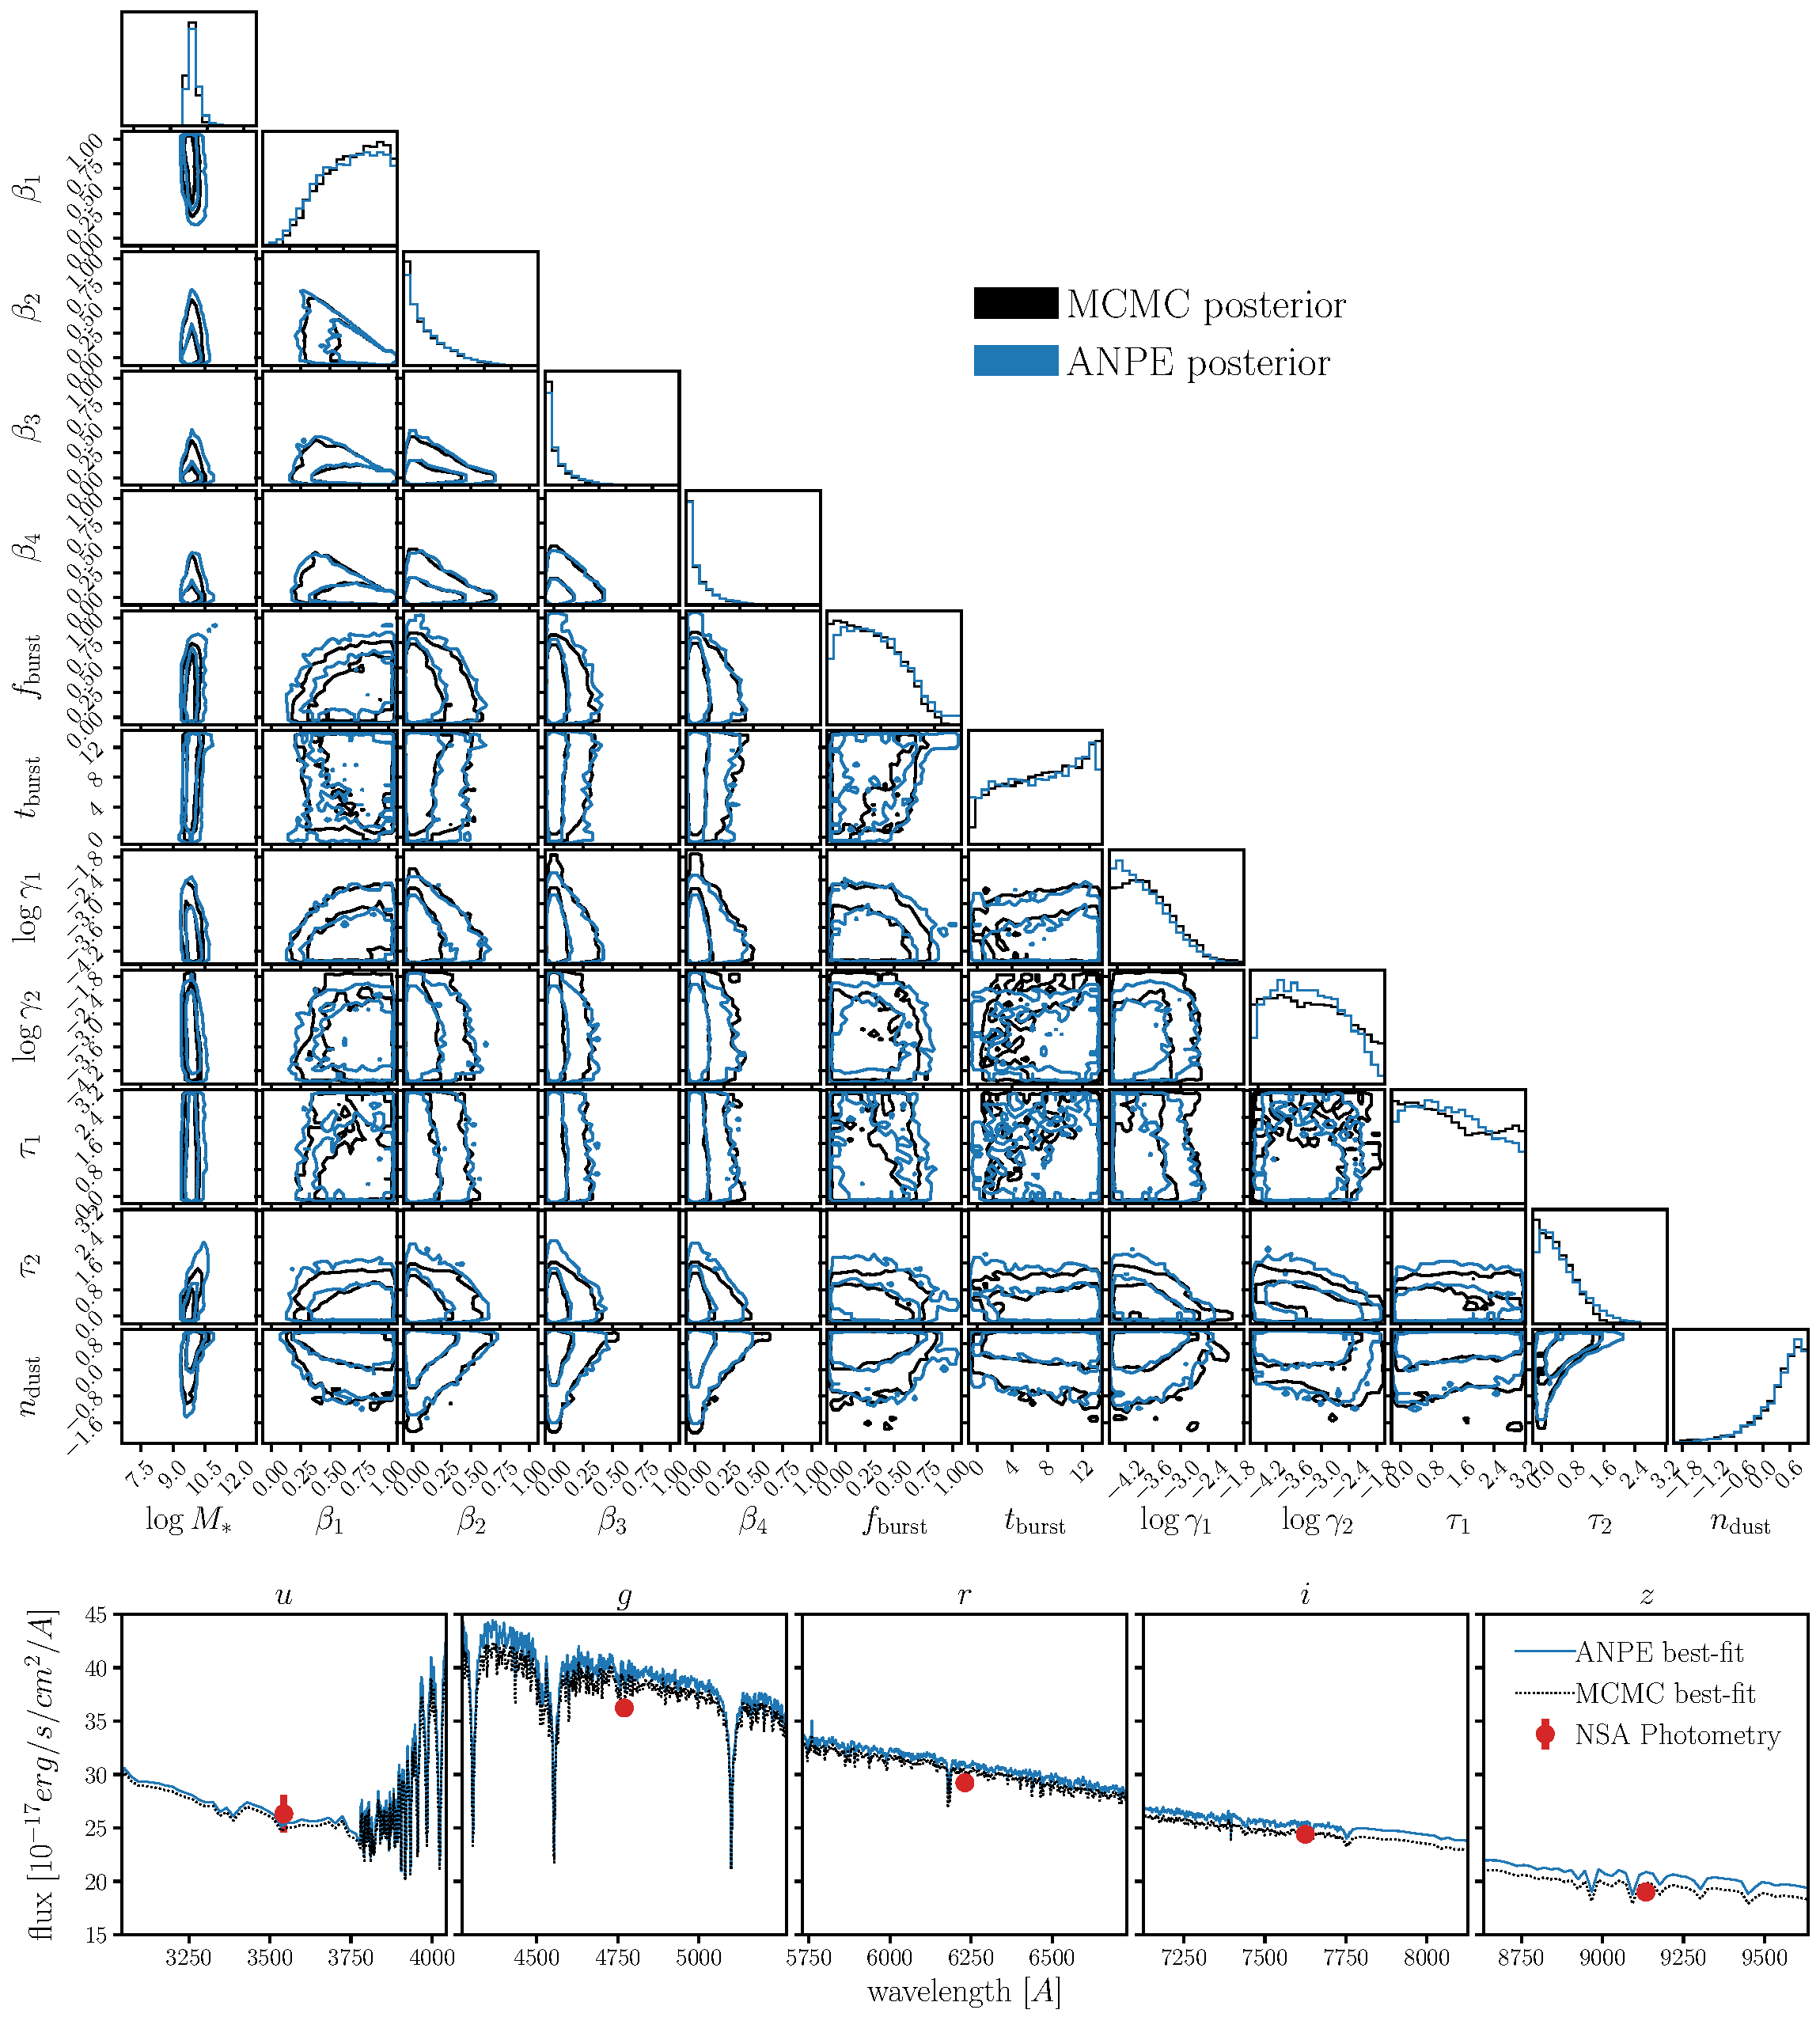
\includegraphics[width=0.9\textwidth]{figs/corner.pdf}
    \caption{\label{fig:corner}
    A comparison of the posteriors of the 12 SED model parameters derived from
    standard MCMC sampling (black) and our ANPE (blue) for a single arbitrarily
    selected NSA galaxy.
    The posteriors are in excellent agreement for all of the parameters. 
    Estimating the posterior using MCMC sampling requires X hours. 
    Even using neural emulators to accelerate likelihood evaluations, MCMC
    sampling requires Y hours. 
    \emph{With ANPE, inferring the full posterior requires 1 second per
    galaxy.}
    }
\end{center}
\end{figure}

\section{Results} \label{sec:results}
Now that we have trained our ANPE, we validate whether the posteriors we infer
using it are accurate.
As a first test, we compare the posterior from ANPE to the posterior derived
from MCMC sampling for a single arbitrarily chosen NSA galaxy in
Figure~\ref{fig:corner}. 
In the top, we present the the posterior distribution of the 12 SED model
parameters (Section~\ref{sec:provabgs}) for the ANPE posterior (blue) and MCMC
posterior (black). 
\emph{The ANPE posterior is in excellent agreement with the MCMC posterior for
all of the SED parameters}. 
 
In the bottom of Figure~\ref{fig:corner}, we compare the SED distributions of
the best-fit parameter values from the ANPE (blue) and MCMC posteriors (black
dotted). 
We also include the NSA photometric flux of the selected galaxy (red) and mark
the optical broadband response curves (dashed). 
The best-fit SED from the ANPE posterior is also in good agreement with both
the MCMC best-fit and the NSA photometry.  

% separate paragraph highlighting the computational advantage? 
The key advantage of ANPE is that it enables accurate Bayesian inference
orders of magnitude faster than conventional methods. 
We derive the MCMC posterior using the {\sc Zeus} ensemble
slice-sampler~\citep{karamanis2020} with 30 walkers and 10,000 iterations.
2,000 of the iterations are discarded for burn-in. 
In total, the MCMC posterior requires >100,000 SED model evaluations. 
Since each evaluation takes ${\sim}340$ ms, it ${\sim}10$ CPU hours for
a single MCMC posterior. 
SED modeling has recently adopted neural emulators to accelerate SED model
evaluations. 
In \chedit{Hahn~\etal~(2022)}, for instance, the PROVABGS emulator takes
${\sim}2.9$ ms to evaluate, $>100\times$ faster than the original model. 
Yet, even with emulators, due to the number of evaluations necessary for
convergence, an MCMC posterior takes ${\sim}10$ CPU minutes. 
Meanwhile, after training, \emph{the ANPE posterior takes $1$ second ---
>$10^5\times$ faster than MCMC}. 

\begin{figure}
\begin{center}
    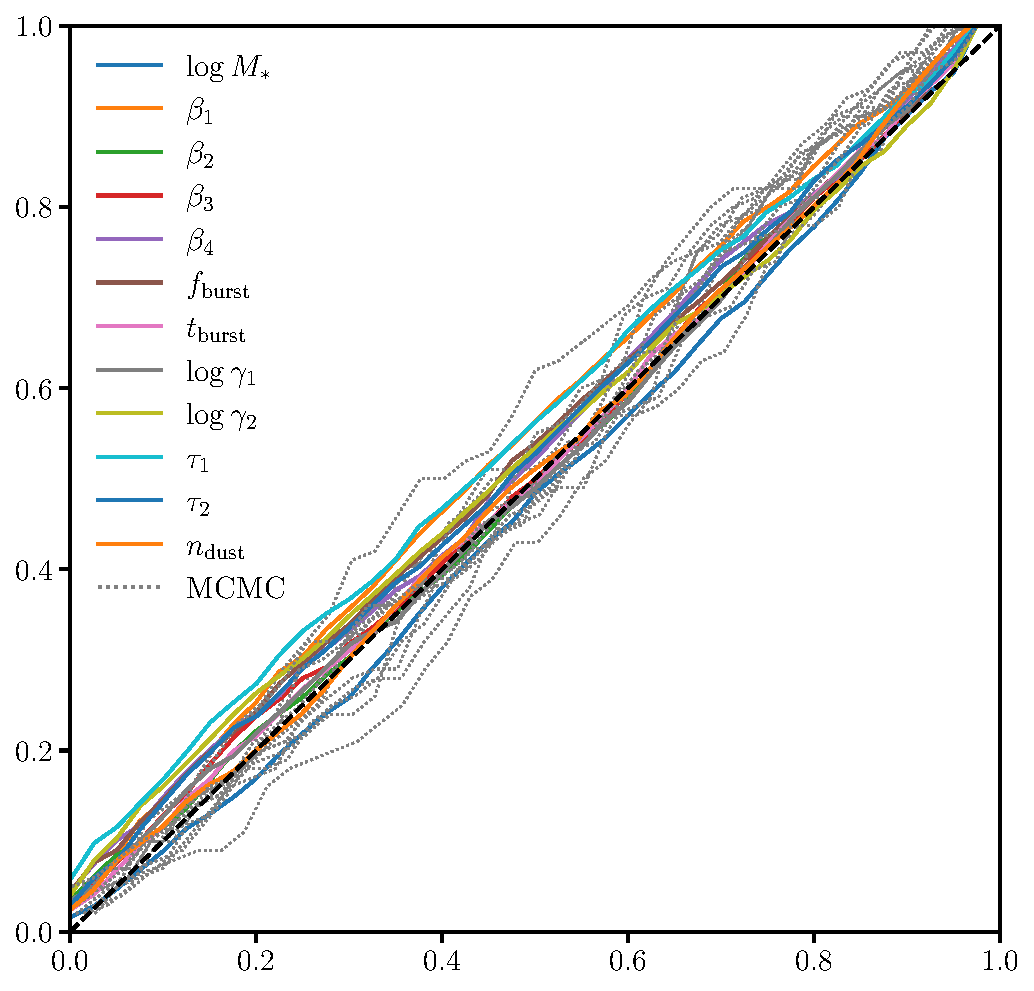
\includegraphics[width=0.5\textwidth]{figs/ppplot.pdf}
    \caption{\label{fig:pp}
    Probability-probability (p-p) plot of the ANPE for 1000 simulated test data. 
    For each SED parameter, we plot the cumulative distribution function (CDF) of the
    percentile score of the true value within the ANPE marginalized posterior.
    For the true posteriors, the percentile score is uniformly distributed so
    the CDF is diagonal (black dashed).
    The test data is constructed in the same way as the training data
    (Section~\ref{sec:training}). 
    For reference, we include the p-p plot of the posterior estimated from MCMC
    sampling (gray). 
    \emph{The ANPE is in good agreement the true posterior.}
    }
\end{center}
\end{figure}
Besides the selected NSA galaxy in Figure~\ref{fig:corner}, the posteriors from
ANPE and MCMC are overall in excellent for NSA galaxies.
However, we do not know the true SED parameters for these galaxies so to
further validate the ANPE posteriors, we use test synthetic photometry, where
we know the truth.
We sample 1000 SED parameters from the prior,
$\{\theta^{\rm test}_i\} \sim p(\theta)$, 
and construct synthetic NSA galaxy photometry, 
$\{{\bf x}^{\rm test}_i\}$, 
for them in the same way as the training data in Section~\ref{sec:training}. 
Afterwards, we generate posteriors for each of test data using our ANPE: 
$\{ p(\theta \given {\bf x}^{\rm test}_i)\}$. 

In Figure~\ref{fig:pp}, we present the probability-probability (p-p) plot of
the ANPE posteriors for the test data. 
The p-p plot presents the cumulative distribution function (CDF) of the
percentile score of the true value within the marginalized posterior for each
SED parameter. 
For the true posterior, the percentiles are uniformly distributed so the CDF
is a diagonal (black dashed).
\emph{Overall, the ANPE posteriors are in good agreement with the true
posteriors for each of the SED parameters}.

We also include in Figure~\ref{fig:pp} the CDFs of the SED parameters for the
MCMC posteriors derived for a subset of 100 test galaxy photometry (gray
dotted). 
Based on the CDFs, the ANPE posteriors are actually in better agreement with
the true posteriors than those derived from MCMC.
This is due to the fact that MCMC posteriors are only estimates of the true
posterior and are subject to limitations in initialization, sampling, and
convergence.
Meanwhile, these limitations do not impact posteriors from ANPE and so the
comparison highlights additional advantages of ANPE besides the $10^5\times$
speed up.

\begin{figure}
\begin{center}
    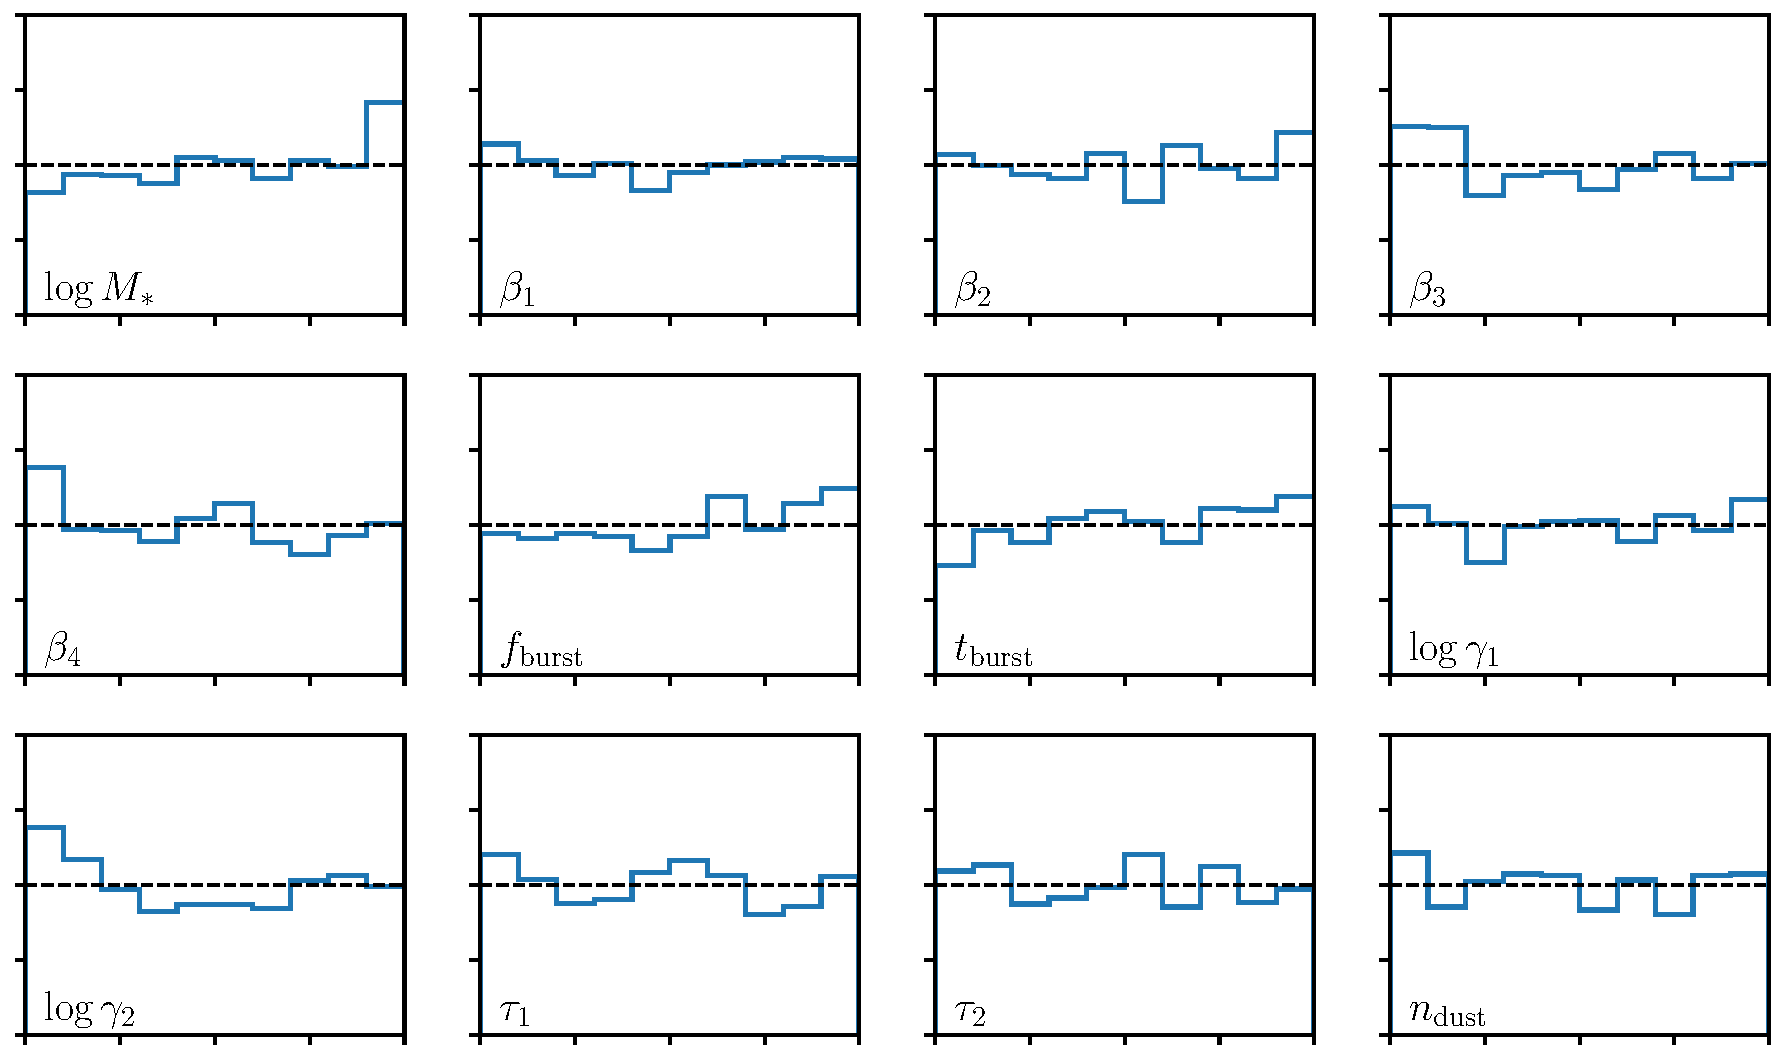
\includegraphics[width=0.9\textwidth]{figs/sbc.pdf}
    \caption{\label{fig:sbc}
    Simulation-based calibration plot of the ANPE for 1000 simulated test data. 
    For each SED parameter, we plot the histogram of the rank statistic of the
    true value within the marginalized ANPE posterior (blue). 
    For the true posterior, the rank statistics will have a uniform
    distribution (black dashed). 
    For reference, we include the rank dstirubtion of the MCMC posterior for a
    subset of 100 test data (gray dotted). 
    \emph{The ANPE is in good agreement the true posterior.}
    }
\end{center}
\end{figure}

We examine another validation of the ANPE posteriors using simulation-based
calibration~\citep[SBC;][]{talts2020}. 
Rather than using percentile scores, SBC examines the distribution of the rank
statistics of the true parameter values within the marginalized posteriors. 
It addresses the fact that the CDFs only asymptotically approach the true
values and that the discrete sampling of the posterior can cause artifacts in
the CDFs. 
In Figure~\ref{fig:sbc}, we present SBC of each SED model parameter for the
ANPE posteriors (blue) using the 1000 test data.
For comparison, we include the SBC for the MCMC posteriors (gray dotted). 
Similar to the percentile score, the distribution of the rank statistic is
uniform for the true posterior (black dashed). 
The distribution of rank statistic for the ANPE posteriors are overall in good
agreement with a uniform distribution. 
Hence, the ANPE posteriors are in good agreement with the true posterior. 

An advantage of SBC is that by examining the deviation of rank statistics
distribution from uniformity, we can determine how the ANPE posteriors deviate
from the true posteriors. 
For most of the SED parameters, we find little deviation from uniformity so the
ANPE posterior is accurate. 
However, we find a noticeable deviation for $\log\gamma_2$, the coefficient of
the second ZH NMF basis function. 
The rank statistic distribution of $\log\gamma_2$ has a symmetric U shape where
the true parameter values are more often at the lowest and highest ranks.
This means that on average the ANPE posterior for $\log\gamma_2$ is narrower
than the true posterior and underestimates the uncertainty. 
To better gauge the actual impact of such a discrepancy, we examine the
distributions of the MCMC posterior.
Since we only use 100 test data for MCMC the distributions are noisy; however,
we find overall significantly large discrepancies from uniformity (see 
\emph{e.g.} $\log M_*$ and $\beta_4$ panels). 
Based on this comparison, we conclude that our ANPE produces posteriors that
are in good agreement with the true posteriors.  
\chedit{revisit once we have the final ANPE} 

With the accuracy of our ANPE validated, we now apply it to derive posteriors
for all of our NSA galaxies (Section~\ref{sec:obs}). 
\todo{elaborate on this} 
We make the 
